\chapter{Parameters for Chemical Kinetics Calculations}

\graphicspath{{./Figures/Kinetics/}}

\section{Introduction to Chemical Kinetics} 
Chemical kinetics calculations are a very useful way to take quantum
chemical results and compare the predictions to experimental
results. With kinetics software one can predict the evolution of large
mixtures of reactants over time, can model combustion and detonation
processes, and can predict equilibrium mixtures. 

In kinetics we're interested in how fast chemical reactions run. Given
a reaction, for example,
\begin{equation}
 \chem{Br} + \chem{H_2} \rightleftharpoons \chem{HBr} + \chem{H},
\end{equation}
how fast are the products (\chem{HBr}) produced? Using simple
kinetics, we can write the rate of product production as a function of
a \emph{rate constant} times the concentrations of the reactants:
\begin{equation}
 \frac{\partial [\chem{HBr}]}{\partial t} =
  k[\chem{Br}][\chem{H_2}].
\end{equation}
For simple reactions like this it is easy to work out the kinetic
equations, and even to integrate them given different starting
conditions. However, reaction networks become complex very
rapidly. The combustion of hydrogen and oxygen to produce water
\begin{equation}
 \chem{H_2} + \chem{O_2} \rightleftharpoons \chem{H_2O}
\end{equation}
has 10 elementary reactions in it. People who model hydrocarbon
combustion routinely deal with reaction networks that have thousands
of reactions. As reaction networks become more complex, we need to use
computer programs to integrate all of the variables
simultaneously. The first part of this chapter discusses the software
used in these simulations and what types of parameters it
requires. The second part of this chapter then examines how quantum
chemistry calculations may be used to determine these parameters.

\section{The Chemkin program and associated parameter files} 
The most commonly used chemical kinetics program is the Chemkin
package, originally developed by Sandia National Laboratories
\cite{chemkin2}, and currently marketed by Reaction Design. Two free
alternatives to the Chemkin package are Cantera \cite{Goodwin02} and
Fuego \cite{Aivazis02}, both being developed at Caltech. Of these
efforts, Cantera is the most mature, and information on the status of
the program may be found at the Cantera web site
\href{http://www.cantera.org}{http://www.cantera.org}.

Given a collection of species \chem{X_1}, \chem{X_2}, \dots, at
concentrations [\chem{X_1}], [\chem{X_2}], \dots and a given
temperature $T$ and pressure $P$, Chemkin determines the rate of
change of these variables $\frac{\partial[\chem{X_i}]}{\partial t}$,
$\frac{\partial T}{\partial t}$, $\frac{\partial P}{\partial
t}$. Although this may seem very straightforward, it enables one to
take a set of initial conditions, and, for example, simulate the
detonation of explosive materials over time, as shown in Figure
\ref{hmx-species}.

\begin{figure}
\begin{center}
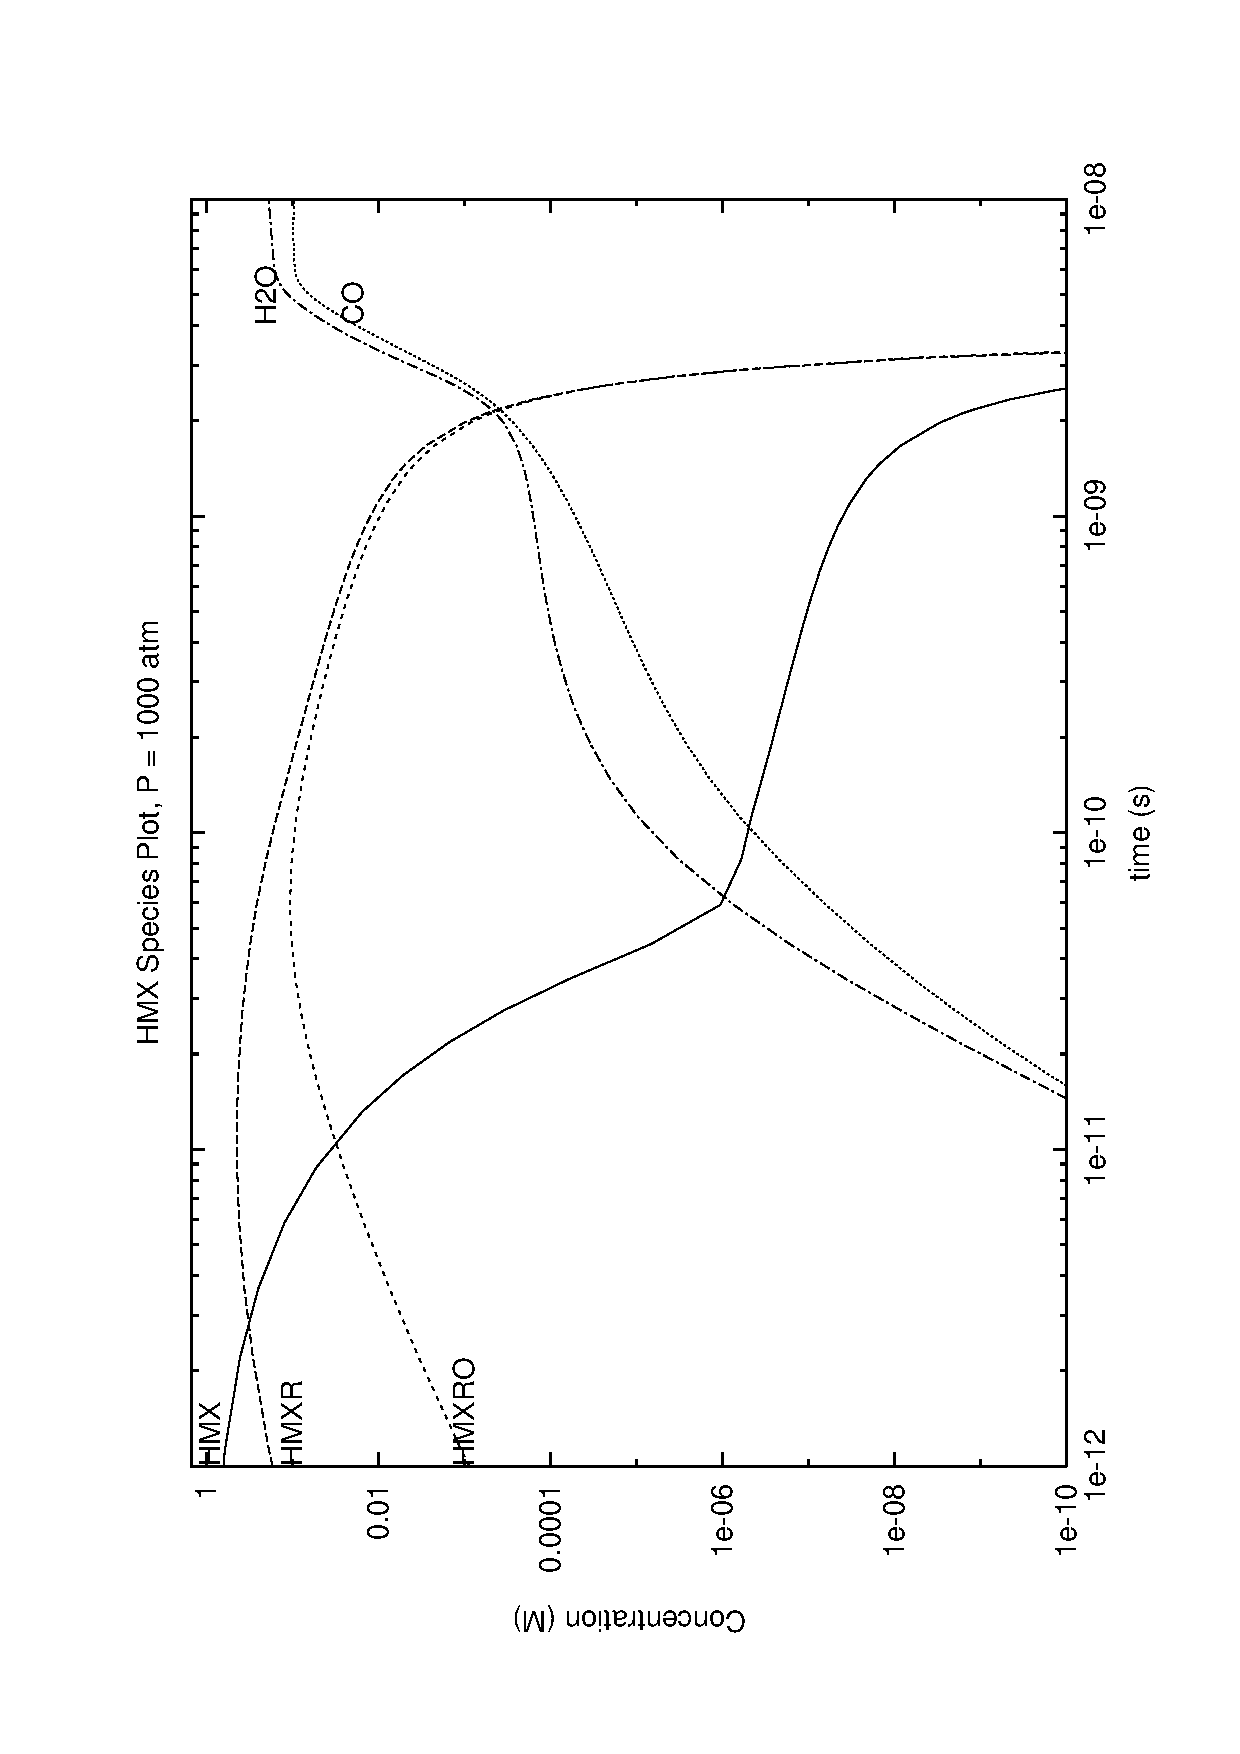
\includegraphics[angle=270,scale=0.5]{hmx-species}
\end{center}
\caption{Detonation of the explosive material HMX over time, computed
using a Chemkin constant volume calculation at P=1000 atm and T=1500
K. The material detonates at $\approx 2\times 10^{-9}$ sec. The
mechanism used to study this process contains over 90 species and 450
reactions, and thus requires a computer program to simulate.}
\label{hmx-species}
\end{figure}

A Chemkin mechanism file has four sections: (i) an elements section
that lists the relevant elements in the reaction; (ii) a species
section that lists all of the species; (iii) a thermochemistry section
that contains composition and thermochemical information for each of
the species; and (iv) a reactions section that describes kinetic
parameters for each reaction.

An example of a species entry for the thermochemistry section is
\begin{verbatim}
C2H2              121386C   2H   2      G  0300   5000  1000  
 0.04436E+02 0.05376E-01-0.01912E-04 0.03286E-08-0.02156E-12
 0.02566E+06-0.02800E+02 0.02013E+02 0.01519E+00-0.01616E-03
 0.09078E-07-0.01912E-10 0.02612E+06 0.08805E+02               
\end{verbatim}
This record is for acetylene, \chem{C_2H_2}. The first record is the
name of the species, and the second record (121386) is an (arbitrary)
identifying number, generally the date on which the data was
generated. The next four records (\verb:C   2H   2:) indicate that
there are 2 carbon and 2 hydrogen atoms in this species. The next
record (\verb:G:) indicates that the species is gaseous, and the next
three records say that the thermochemical data is fit from 300--5000
K, and that the turnover point from the low-temperature to the
high-temperature regime is 1000 K.

The next 14 records are parameters for the \emph{NASA thermochemical
polynomial fit} to the thermochemical data, given by
\begin{eqnarray}
C_p/R &=& a_1 + a_2T + a_3T^2 + a_4T^3 + a_5T^4\\
H/RT &=& a_1 + a_2T/2 + a_3T^2/3 + a_4T^3/4 + a_5T^4/5 + a_6/T\\
S/R &=& a_1\ln T + a_2T + a_3T^2/2 + a_4T^3/3 + a_5T^4/4 + a_7
\end{eqnarray}
The first 7 records contain $a_1$--$a_7$ for the high temperature
range, and the next 7 records contain $a_1$--$a_7$ for the low
temperature range.  To determine parameters for these polynomials, the
techniques of Chapter \ref{chap-thermochem} are used to compute the
heat capacity $C_p$, the enthalpy $H$, and the entropy $S$ over a wide
range of temperatures. These data are then fit using a standard set of
programs to the NASA thermochemical form. Figure \ref{hmx-therm} shows
representative data for the energetic material HMX and the NASA fit to
these data.

\begin{figure}
\begin{center}
\includegraphics[scale=0.5,angle=270]{hmx.eps}
\end{center}
\caption{HMX molecule thermodynamic data for $C_p$ and $S$ from DFT
calculation (points) and fit to NASA polynomial (lines), in cal/mol K.}
\label{hmx-therm}
\end{figure}

\begin{table}
\caption{Examples of reaction parameters in a Chemkin mechanism.}
\label{chemkin-reaction}
\begin{center}
\begin{tabular}{llll}\hline\hline
Reaction & A & $\beta$ & $E_a$ \\ \hline
$\chem{O}+\chem{H_2}\rightleftharpoons \chem{H}+\chem{OH}$       
 & 5.000E+04 &  2.670 &  6290.00\\
$\chem{O}+\chem{HO_2}\rightleftharpoons \chem{OH}+\chem{O_2}$     
 & 2.000E+13 &   .000 &      .00\\ 
$\chem{O}+\chem{H_2O_2}\rightleftharpoons \chem{OH}+\chem{HO2}$   
 & 9.630E+06 &  2.000 &  4000.00\\
\hline\hline
\end{tabular}
\end{center}
\end{table}


Table \ref{chemkin-reaction} shows typical reactions from the
reactions section of the Chemkin file. The basic information contains
the species in the reaction, and $A$, $\beta$, and $E_a$ parameters
for the \emph{modified Arrhenius equation}
\begin{equation}
 k=AT^\beta\exp\{-E_a/k_bT\}
\end{equation}
where $A$ is the \emph{pre-exponential factor}, $T$ is the temperature
of the reaction, $\beta$ is the temperature exponent, $E_a$ is the
\emph{activation energy}, and $k_b$ is Boltzmann's constant.

In many dissociation or recombination reactions a \emph{third body} is
required to carry off excess kinetic energy. In Chemkin reactions
these processes are normally written as
\begin{equation}
 \chem{H} + \chem{O_2} + \chem{M} \rightleftharpoons \chem{HO_2} + \chem{M}
\end{equation}
where the species \chem{M} represents a generic third body species. It
is often the case that some species act more efficiently than others
as a third body, and then the \emph{third body efficiency} is
specified as, for example,
\begin{verbatim}
 H2/ 2.40/ H2O/15.40/ CH4/ 2.00/
\end{verbatim}

Another type of specification commonly made in Chemkin mechanism files
is the \emph{pressure-dependent fall-off reaction}
parameters. Consider the recombination reaction of two methyl
radicals. In the high-pressure regime, the appropriate reaction is
$\chem{CH_3}+\chem{CH_3}\rightleftharpoons\chem{C_2H_6}$. In the
low-pressure regime, the appropriate reaction is 
$\chem{CH_3}+\chem{CH_3}+\chem{M}\rightleftharpoons\chem{C_2H_6}+M$.
The regime between these two limits is known as the fall-off regime.
Chemkin keywords \verb:LOW: and \verb:TROE: specify parameters for
different types of treatments of these regimes.

%Constant Volume calculations

%Sensitivity analysis

\section{Conventional Transition State Theory}
We now want to understand how to use the quantum chemistry techniques
we have developed in this course to compute parameters to be used in
chemical kinetics calculations.
How can we go from static
properties of the energy at different geometries to obtain intuition
about the reaction dynamics of the system? We will use conventional
transition state theory (CTST). CTST is built upon four major
assumptions
\begin{enumerate}
\item Molecular systems that have surmounted the saddle point in the
direction of products cannot turn back and form reactants again.
\item The energy distribution among the reactants follows the
Maxwell-Boltzmann distribution, and thus the concentration of
activated complexes may be computed from equilibrium theory.
\item The motion along the reaction path is separable from the other
motions of the activated complex.
\item A chemical reaction may be treated classically, with quantum
effects such as tunneling ignored.
\end{enumerate}
There are many different ways to express CTST. The way that we will
find the most convenient is known as the \emph{thermodynamic
formulation}. 
\begin{equation}
 k = \frac{k_BT}{h}\exp\{-\Delta G^\ddag/RT\}
\label{tst}
\end{equation}
Here $k_B$ is the Boltzmann constant ($1.38066\times 10^{-23}
JK^{-1}$), $T$ is the temperature, $h$ is Planck's constant
($6.62618\times 10^{-34} Js$), $R$ is the ideal gas constant ($2 cal
mol^{-1}K^{-1}$), and $\Delta G^\ddag$ is the free energy change
between the ground state and the transition state. The prefactor
$\frac{k_BT}{h}$ has units of $s^{-1}$, and we can think of it as how
rapidly the reactant tries to cross the barrier. The exponential term
$\exp\{-\Delta G^\ddag/RT\}$ is dimensionless, and we can think of it
as how easy it is to get over the barrier. When we multiply the two
terms together we get a good estimate of the ease at which the barrier
may be crossed.


\begin{figure}
\begin{center}
\includegraphics[scale=0.5]{h3-isom.eps}
\end{center}
\caption{Schematic drawing of the \chem{H_2}+\chem{H} atom transfer reaction.}
\label{h3-isom}
\end{figure}

As an example of how CTST may be used, we consider the reaction
$\chem{H_2}+\chem{H}\rightleftharpoons\chem{H}+\chem{H_2}$, shown
schematically in Figure \ref{h3-isom}. We first compute the ground and
transition state geometries and energies. It turns out that there is
an energy difference of 5.99 kcal/mol between the ground and
transition state. We also use the techniques described in section
\ref{chap-thermochem} to approximate the free energy at a variety of
temperatures. Table
\ref{h3-data-table} presents the raw data that we will use for our
plot.

\begin{table}
\caption{Data for computing kinetics parameters for the
\chem{H_2}+\chem{H} reaction.}
\label{h3-data-table}
\begin{center}
\begin{tabular}{ccccccccc}\\ \hline\hline
$T$ & $E^0$ & $G^0$ & $E^\ddag$ & 
 $G^\ddag$ & $\Delta G^\ddag$& $1000/T$ & $k$ & $\ln(k)$ \\ \hline
0      & 0 & 6.74   & 5.99 & 11.86  & 5.12 \\ 
298.15 & 0 & -3.36  & 5.99 &  3.19  & 6.56  & 3.354 &
 $9.69\times 10^7$ & 18.39    \\ 
398.15 & 0 & -8.01  & 5.99 & -0.54  & 7.47  & 2.512 &
 $6.59\times 10^8$ & 20.31    \\ 
498.15 & 0 & -12.96 & 5.99 & -4.50  & 8.47  & 2.007 &
 $2.00\times 10^9$ & 21.42    \\ 
598.15 & 0 & -18.15 & 5.99 & -8.64  & 9.52  & 1.672 &
 $4.15\times 10^9$ & 22.15    \\ 
698.15 & 0 & -23.54 & 5.99 & -12.94 & 10.60 & 1.432 &
 $6.97\times 10^9$ & 22.66    \\ 
\hline\hline
\end{tabular}
\end{center}
\end{table}


Our goal is to fit these data to an \emph{Arrhenius equation}
\begin{equation}
 k = A\exp\{-E_a/RT\}.
\end{equation}
What we are doing here is effectively removing the temperature
dependence of the preexponential factor in the CTST rate expression.
Because chemists have been doing these calculations since long before
there were computers to analyze them they developed a convenient way
to obtain the relevant factors. One makes an \emph{Arrhenius plot}
whereby $\ln(k)$ is plotted as a function of $1000/T$. The
$y$-intercept of the plot gives $\ln{A}$, and the slope of the plot
gives $E_a/1000R$, which means that we can determine $A$ and $E_a$
with only graph paper and a ruler rather than a computer (but as long
as we have one, we may as well use it). Table \ref{h3-data-table} also
has columns that convert the \chem{H_2}+\chem{H} data to the proper
form for plotting, using equation \ref{tst} to estimate the
rate. Figure \ref{h2-h-arrhen} shows the Arrhenius plot of these data,
along with the straight line fit that yields $E_a=4.42 kcal/mol$ and
$A=1.7\times 10^{11}$. 

\begin{figure}
\begin{center}
\includegraphics[scale=0.5,angle=270]{h2-h-arrhen.eps}
\end{center}
\caption{\chem{H_2}+\chem{H} Arrhenius plot, showing the data from
table \ref{h3-data-table} (points) fit to an Arrhenius equation
(line). The data in this plot yields $E_a=4.42$ kcal/mol and
$A=1.7\times 10^{11}$.}
\label{h2-h-arrhen}
\end{figure}

Before we leave this very simple reaction, let us consider a great
simplification of the preexponential factor that is due to (USC
professor) Sidney Benson. For bimolecular reactions, Benson estimated
that the prefactor was given by
\begin{equation}
 A = \frac{k_BT}{h}\exp\{-\Delta S^\ddag/R\}
\end{equation}
where now $\Delta S^\ddag$ is the entropy change between the reactant
state and the transtition state. Using this approximation for the 
\chem{H_2}+\chem{H} reaction just studied yields a preexponential
factor of $A = 2.3\times 10^{11}$, in remarkable agreement with the
more accurate value.

\begin{figure}
\begin{center}
\includegraphics[scale=0.5]{h-recomb.eps}
\end{center}
\caption{The free energy $G$ pathway can have a barrier even for
reactions such as radical recombination where the energy $E$ has no
barrier.}
\label{h-recomb}
\end{figure}

Lorant and Goddard have also shown that we can use transition state
theory techniques to obtain rate constants for barrierless
reactions. Consider the reaction hydrogen atom recombination reaction
$\chem{H} + \chem{H} \rightleftharpoons \chem{H_2}$. The reaction has
no barrier, and traditionally people have assumed that treatment of
this reaction with transition state theory was impossible. Lorant and
Goddard showed that even when the reaction energy had no barrier, it
was still possible to find a barrier along the free energy pathway,
and that the same transition state theory could be used to determine
the rate constants for these reactions. Figure \ref{h-recomb} shows a
(greatly exaggerated) schematic of exactly how this would work. Lorant
and Goddard's technique is a breakthough because it allows rate
constants to be determined for reactions that could only otherwise be
computed using expensive RRKM techniques.

\section{Calculation of Rate Constants for Unimolecular Reactions}
The calculations we discussed in the previous section are
inadequate for describing unimolecular processes. Fortunately, a
number of excellent treatments of unimolecular reactions have been
developed over the years, culminating in RRKM theory, developed by
Rice, Ramsberger, Kassel, and Marcus. A full treatment of RRKM theory
is beyond the scope of the current work, but we will present a brief
overview here.

\begin{figure}
\begin{center}
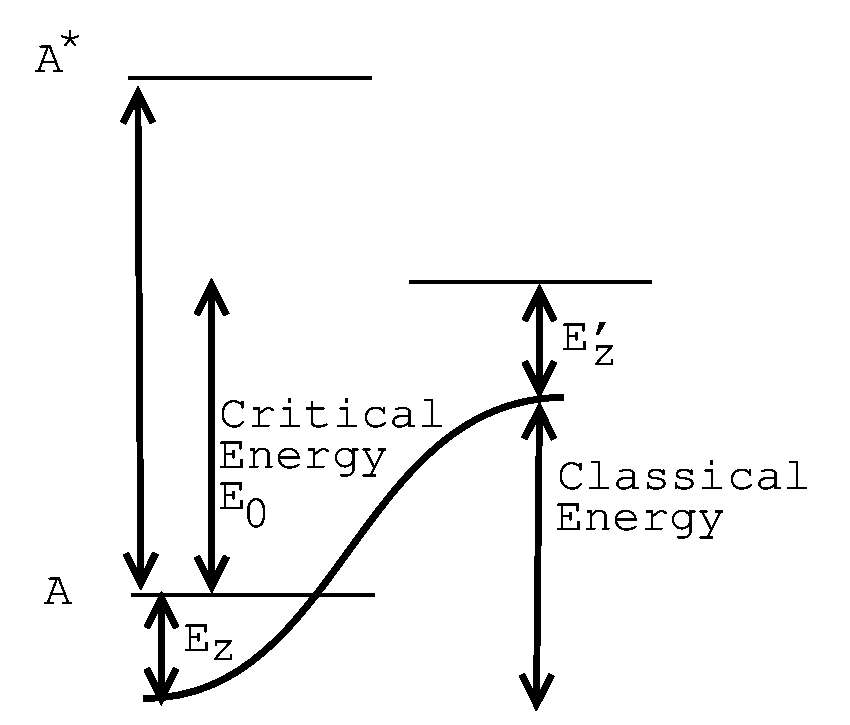
\includegraphics[scale=0.5]{rrkm.eps}
\end{center}
\caption{Energies involved in RRKM calculations. The classical energy
is corrected by the zero-point energies of the ground and transition
states. The molecule \chem{A} is excited to some energized species
\chem{A^*} that has more energy than the critical energy for reaction,
$E_0^*$.}
\label{rrkm}
\end{figure}

RRKM theory assumes that unimolecular reactions proceed according to
\begin{eqnarray}
 \chem{A} + \chem{M} &\stackrel{k_1}{\rightleftharpoons}& 
   \chem{A^*} + \chem{M}\\
 \chem{A^*} &\stackrel{k_2}{\rightarrow}& \chem{B}+\chem{C}
\end{eqnarray}
where the molecule \chem{A} is excited by collision with inert species
\chem{M} to some \emph{energized complex} \chem{A^*} which can then
react to form products \chem{B} and \chem{C}. Figure \ref{rrkm} shows
some the energies that enter into such a process.

By standard steady state theory we could assume
\begin{equation}
 k = \frac{k_2(k_1/k_{-1})}{1+k_2/k_{-1}[M]}.
\end{equation}
In RRKM we recognize that both $k_2$ and $f=k_1/k_{-1}$ are functions
of the energy $E^*$. Thus, in differential form
\begin{equation}
 dk = \frac{k_2(E^*)f(E^*)}{1+k_2(E^*)/k_{-1}[M]}dE^*.
\end{equation}
and in integral form
\begin{equation}
 k = \int_{E_0^*}^{\infty}\frac{k_2(E^*)f(E^*)}{1+k_2(E^*)/k_{-1}[M]}dE^*.
\end{equation}
The distribution function $f(E^*)$ is given by
\begin{equation}
 f(E^*)dE^* = \frac{N(E^*)\exp\{-E^*/kT\}dE^*}
  {\int_0^\infty N(E^*)\exp\{-E^*/kT\}dE^*}
\end{equation}
where $N(E^*)$ is the density of states with energies between $E^*$
and $E^*+dE^*$. The expression for $k_2(E^*)$ is given by
\begin{equation}
 k_2(E^*) = \frac{l^\ddag\sum E_\mathrm{active}^*}{hN(E^*)F_r}
\end{equation}
where $l^\ddag$ is the statistical factor, the ratio of the number of
symmetrically identical products to the number of symettrically
identical reactants, $P(E)$ is the number of rovibrational states of
the activated molecule up to $E$, and $F_r$ is a scaling factor to
account for the fact that the rotations are not the same in the
energized and the activated structures.

The \verb:UNIMOL: program is the most commonly used programs to do
RRKM calculations.

